\documentclass[a4paper]{article}
\usepackage[utf8]{inputenc}
\usepackage[fontsize=12pt]{scrextend} % set fontsize 13pt
\usepackage[T5]{fontenc} % viet tieng viet
\usepackage{fancyhdr}
\usepackage{booktabs}
\usepackage{amsmath}
\usepackage{lastpage}
\usepackage[lined,boxed,commentsnumbered]{algorithm2e}
\usepackage{enumerate}
\usepackage{color}
\usepackage{graphicx}							% Standard graphics package
\usepackage{array}
\usepackage{tabularx, caption}
\usepackage{multirow}
\usepackage[framemethod=tikz]{mdframed}% For highlighting paragraph backgrounds
\usepackage{multicol}
\usepackage{rotating}
\usepackage{graphics}
\usepackage{geometry}
\usepackage{setspace}
\usepackage{epsfig}
\usepackage{tikz}
\usepackage{listings}
\usetikzlibrary{arrows,backgrounds}
\usepackage{hyperref}
\usepackage{titlesec}
\usepackage{float} 

\newlength{\mylistingwidth}

\lstset{
    basicstyle=\color{white}\ttfamily,
    backgroundcolor=\color{black},
    keywordstyle=\color{white},
    columns=fullflexible,
    linewidth=\mylistingwidth,
    language=bash
}

\titlespacing*{\section}{0pt}{0pt}{10pt} % Heading 1
\titleformat*{\section}{\fontsize{16pt}{0pt}\selectfont \bfseries \centering}

\hypersetup{urlcolor=blue,linkcolor=black,citecolor=black,colorlinks=true} 
%\usepackage{pstcol} 								% PSTricks with the standard color package

\everymath{\color{blue}}
\usepackage{fancyhdr}
\setlength{\headheight}{29.49261pt}
\addtolength{\topmargin}{-30pt}

\pagestyle{fancy}
\fancyhead{} % clear all header fields
\fancyhead[L]{
 \begin{tabular}{rl}
    \begin{picture}(25,15)(0,0)
    \put(0,-8){
\includegraphics[width=8mm, height=8mm]{images/logoITSGUsmall.png}}
    %\put(0,-8){\epsfig{width=10mm,figure=hcmut.eps}}
   \end{picture}&
	%\includegraphics[width=8mm, height=8mm]{hcmut.png} & %
	\begin{tabular}{l}
		\textbf{\bf \ttfamily Trường Đại học Sài Gòn}\\
		\textbf{\bf \ttfamily Khoa Công Nghệ Thông Tin}
	\end{tabular} 	
 \end{tabular}
}
\fancyhead[R]{
	\begin{tabular}{l}
		\tiny \bf \\
		\tiny \bf 
	\end{tabular}  }
\fancyfoot{} % clear all footer fields
\fancyfoot[L]{\scriptsize \ttfamily Bài tập lớn môn Phát triển phần mềm mã nguồn mở - Niên khóa 2024-2025}
\fancyfoot[R]{\scriptsize \ttfamily Trang {\thepage}/\pageref{LastPage}}
\renewcommand{\headrulewidth}{0.3pt}
\renewcommand{\footrulewidth}{0.3pt}
\renewcommand{\contentsname}{} % Loại bỏ tiêu đề của mục lục

%%%
% \setcounter{secnumdepth}{4}
% \setcounter{tocdepth}{3}
% \makeatletter
% \newcounter {subsubsubsection}[subsubsection]
% \renewcommand\thesubsubsubsection{\thesubsubsection .\@alph\c@subsubsubsection}
% \newcommand\subsubsubsection{\@startsection{subsubsubsection}{4}{\z@}%
% {-3.25ex\@plus -1ex \@minus -.2ex}%
% {1.5ex \@plus .2ex}%
% {\normalfont\normalsize\bfseries}}
% \newcommand*\l@subsubsubsection{\@dottedtocline{3}{10.0em}{4.1em}}
% \newcommand*{\subsubsubsectionmark}[1]{}
% \makeatother

% \definecolor{dkgreen}{rgb}{0,0.6,0}
% \definecolor{gray}{rgb}{0.5,0.5,0.5}
% \definecolor{mauve}{rgb}{0.58,0,0.82}

\begin{document}

\begin{titlepage}
\begin{center}
TRƯỜNG ĐẠI HỌC SÀI GÒN \\
KHOA CÔNG NGHỆ THÔNG TIN
\end{center}
\vspace{1cm}

\begin{figure}[h!]
\begin{center}

\includegraphics[width=3cm]{images/logoITSGU.png}
\end{center}
\end{figure}

\vspace{1cm}


\begin{center}
\begin{tabular}{c}
	\multicolumn{1}{l}{\textbf{{\Large PHÁT TRIỂN PHẦN MỀM MÃ NGUỒN MỞ}}}\\
	~~\\
	\hline
	\\
	\multicolumn{1}{l}{\textbf{{\Large Xây dựng ứng dụng game 2 người chơi}}}\\
	\\
	
	\textbf{{\Huge Caro trên PYTHON}}\\
	\\
	\hline
\end{tabular}
\end{center}

\vspace{3cm}

\begin{table}[h]
\begin{tabular}{rrl}
\hspace{5 cm} & GVHD: &Từ Lãng Phiêu\\
& SV: & Nguyễn Văn Tiến Dũng - 3120410084\\
& & Lai Quang Vinh - 3120410613 \\

\end{tabular}
\vspace{1.5 cm}
\end{table}

\begin{center}

{\footnotesize TP. HỒ CHÍ MINH, THÁNG 4/2024}
\end{center}
\end{titlepage}

\thispagestyle{empty}

\newpage
\section*{MỤC LỤC}
\tableofcontents
\newpage
\section*{GIỚI THIỆU}

\begin{quotation}
Trò chơi Caro - một trò chơi với nguồn gốc từ trò chơi gomoku cổ điển, nổi tiếng với tên gọi "Five in a Row", là một trong những trò chơi chiến thuật thú vị và sâu sắc. Với lịch sử hơn một thế kỷ, Caro không chỉ là một trò chơi giải trí, mà còn là một bài toán chiến thuật được nhiều người yêu thích và tìm hiểu.

Trò chơi Caro đòi hỏi người chơi phải có sự tư duy chiến thuật, khả năng dự đoán và phản ứng nhanh nhạy. Trên bàn cờ $15 \times 15$, hai người chơi sẽ thay phiên nhau đánh dấu X hoặc O trên các ô trống, với mục tiêu tạo thành một dãy liên tiếp gồm 5 dấu X hoặc O theo hàng ngang, cột dọc hoặc đường chéo.

Trò chơi Caro đã trở thành một biểu tượng văn hóa và là một phần không thể thiếu trong cuộc sống hàng ngày của nhiều người. Không chỉ là một trò chơi giải trí, Caro còn là một nền tảng để thể hiện sự sáng tạo, suy luận và chiến thuật của người chơi.

Trong phiên bản Python của trò chơi Caro, người chơi sẽ trải nghiệm cảm giác hồi hộp khi đối đầu với một người chơi khác qua mạng. Bằng cách sử dụng thư viện đồ họa hoặc giao diện dòng lệnh, chúng ta có thể tạo ra giao diện đồ họa hoặc dòng lệnh thân thiện để người chơi có thể tham gia vào trò chơi một cách dễ dàng.

Caro không chỉ là một trò chơi, mà còn là một cách để kết nối và tạo ra những kỷ niệm đáng nhớ giữa các người chơi. Hãy chuẩn bị tinh thần và tham gia vào thế giới thú vị của trò chơi Caro ngay hôm nay!
\end{quotation}

\newpage

\section*{PHẦN 1: CƠ SỞ LÝ THUYẾT}
\addcontentsline{toc}{section}{PHẦN 1: CƠ SỞ LÝ THUYẾT} % Thêm mục vào mục lục tự động
\setcounter{section}{1}
\subsection{Ngôn ngữ Python}
\subsubsection{Giới thiệu về ngôn ngữ python}
Python là một ngôn ngữ lập trình bậc cao cho các mục đích lập trình đa năng, do Guido van Rossum tạo ra và lần đầu ra mắt vào năm 1991. Python là ngôn ngữ có hình thức rất sáng sủa, cấu trúc rõ ràng, thuận tiện cho người mới học lập trình và là ngôn ngữ lập trình dễ học; được dùng rộng rãi trong phát triển trí tuệ nhân tạo. Cấu trúc của Python còn cho phép người sử dụng viết mã lệnh với số lần gõ phím tối thiểu.
\subsubsection{Ưu điểm của Python}
Là một ngôn ngữ mạnh mẽ và phổ biến hiện nay, Python mang lại nhiều ưu điểm với người dùng như:
\vspace{-5pt}
\begin{itemize}
    \item \textbf{Dễ học và dễ đọc:} Python có cú pháp đơn giản và rõ ràng, giúp việc học và hiểu ngôn ngữ này trở nên dễ dàng cho người mới học lập trình. Cú pháp gọn nhẹ cũng giúp code Python dễ đọc và dễ bảo trì.
    \item \textbf{Hỗ trợ thư viện phong phú:} Python có một cộng đồng lớn và nhiều thư viện phát triển, cung cấp các công cụ và chức năng đa dạng để giải quyết các vấn đề khác nhau.
    \item \textbf{Đa nền tảng: } Python là ngôn ngữ đa nền tảng, có thể chạy trên nhiều hệ điều hành như Windows, macOS và Linux. Điều này giúp xây dựng ứng dụng di động và máy tính để bàn trở nên linh hoạt và dễ dàng.
    \item \textbf{Hỗ trợ cho nhiều lĩnh vực: } Python không chỉ giới hạn trong một lĩnh vực cụ thể. Nó có thể được sử dụng trong phát triển web, phân tích dữ liệu, trí tuệ nhân tạo, trò chơi, mạng, và nhiều lĩnh vực khác.
    \item \textbf{Tích hợp và mở rộng: } Python có khả năng tích hợp tốt với các ngôn ngữ khác như C, C++, và Java bằng cách đó chúng ta có thể tích hợp các module mở rộng để tăng hiệu năng hoặc sử dụng các thư viện bên thứ ba đã có sẵn.
    \item \textbf{Giảm chi phí bảo trì: } Do tính đơn giản của nó, Python giúp bảo trì ứng dụng dễ dàng hơn và do đó, giảm chi phí liên quan, đây là một lợi thế lớn.
\end{itemize}
\subsubsection{Nhược điểm của Python}
\hspace{15pt}
Bên cạnh những ưu điểm kể trên thì Python vẫn có những hạn chế riêng như:
\begin{itemize}
    \item \textbf{Chậm hơn so với ngôn ngữ biên dịch:} Python là ngôn ngữ thông dịch, do đó thường chạy chậm hơn so với ngôn ngữ biên dịch như C++ hoặc Java.
    \item \textbf{Tiêu thụ bộ nhớ lớn: } Các cấu trúc của Python đòi hỏi nhiều không gian bộ nhớ hơn. Ngôn ngữ này không thích hợp để sử dụng cho sự phát triển trong điều kiện bộ nhớ hạn chế.
    \item \textbf{Phát hiện lỗi trong mã: } Vì Python được thực thi thông qua trình thông dịch thay vì trình biên dịch, nên không thể phát hiện lỗi trong quá trình biên dịch.
    \item \textbf{Hạn chế thiết kế: } Python không cung cấp một giao diện người dùng đồ họa (GUI) tiêu chuẩn vì vậy có thể gây ra một số khó khăn trong việc phát triển giao diện người dùng phức tạp.
    \item \textbf{Khó kiểm tra: } Vì nó là một ngôn ngữ dựa trên trình thông dịch, rất khó để chạy các bài kiểm tra trên mã được viết bằng Python. Tất cả các lỗi chỉ xuất hiện trong thời gian chạy, điều này khiến việc kiểm tra các đoạn mã được viết bằng Python rất khó khăn.
\end{itemize}

\subsection{Các thư viện chính đã được sử dụng}
\subsubsection{pygame}
\begin{par}
    Pygame là một thư viện của ngôn ngữ lập trình Python và là một tập hợp các mô-đun Python được thiết kế riêng để lập trình trò chơi. Pygame được viết bởi Pete Shinners và phát hành chính thức từ nằm 2000. Pygame có thể chạy trên nhiều nền tảng và hệ điều hành khác nhau. Với thư viện pygame trong Python, các nhà phát triển có thể sử dụng công cụ và chức năng mở rộng để tạo ra các trò chơi ấn tượng. Bởi vậy, Pygame đang ngày càng phổ biến với nhà phát triển vì tính đơn giản, linh hoạt, dễ sử dụng.
\end{par}

\begin{par}
\textbf{Ưu điểm:}
\begin{itemize}
    \item \textbf{Dễ học và sử dụng: } Pygame được thiết kế để dễ dàng tiếp cận cho người mới học và người mới bắt đầu phát triển game. Cú pháp đơn giản và tài liệu phong phú giúp người dùng nhanh chóng làm quen với thư viện.
    \item \textbf{Đa nền tảng:} Pygame có sẵn trên nhiều nền tảng khác nhau, bao gồm Windows, macOS và Linux. Điều này cho phép bạn phát triển game và ứng dụng đa nền tảng một cách dễ dàng.
    \item \textbf{Hỗ trợ đồ họa và âm thanh:} Pygame cung cấp các chức năng mạnh mẽ để vẽ đồ họa, xử lý hình ảnh, và phát nhạc, âm thanh trong game. Bạn có thể tạo ra các hiệu ứng hình ảnh và âm thanh đa dạng để làm cho game của bạn sống động hơn.
    \item \textbf{Cộng đồng hỗ trợ lớn:} Pygame có một cộng đồng đông đảo và năng động. Bạn có thể tìm thấy nhiều tài liệu, hướng dẫn và nguồn tài nguyên sẵn, ngoài ra người dùng cũng có thể chia sẻ và trao đổi ý tưởng, mã nguồn, và góp ý với nhau từ cộng đồng này.
\end{itemize}
\vspace{10pt}

\textbf{Nhược điểm:}
    \begin{itemize}
    \item \textbf{Hiệu suất hạn chế:} Pygame không phải là một thư viện đồ họa chuyên nghiệp và không được tối ưu hóa để đạt hiệu suất tốt nhất. Điều này có thể gây ra hạn chế về hiệu suất khi xử lý các trò chơi có yêu cầu đồ họa và xử lý phức tạp.
    \item \textbf{Thiếu tính năng cao cấp:} So với một số thư viện phát triển game khác, pygame có thể thiếu một số tính năng cao cấp như hỗ trợ 3D, công cụ phân tích va chạm phức tạp, và hỗ trợ đa luồng mạnh mẽ.
    \item \textbf{Giao diện người dùng hạn chế:} Pygame không cung cấp sẵn các thành phần giao diện người dùng đồ họa (GUI) phức tạp. Bạn cần phải xây dựng và tùy chỉnh giao diện người dùng của mình bằng cách sử dụng các phương pháp và công cụ khác.
\end{itemize}
\end{par}

\subsubsection{pygame-menu}
\begin{par}
    Pygame-menu là một thư viện mã nguồn mở được phát triển cho Python và cung cấp các công cụ để tạo ra các menu và giao diện người dùng cho trò chơi sử dụng thư viện pygame. Với pygame-menu, việc tạo menu đa cấp, các nút tùy chỉnh, và các hiệu ứng chuyển động trở nên dễ dàng và linh hoạt hơn bao giờ hết. Pygame-menu được thiết kế để tích hợp dễ dàng với pygame, cho phép bạn sử dụng các thành phần của pygame để tạo ra các trò chơi đa dạng và phong phú về giao diện người dùng. Nó cũng được hỗ trợ bởi một cộng đồng phát triển động, với nhiều đóng góp và hỗ trợ từ các nhà phát triển khác nhau trên toàn thế giới. Tuy nhiên, tài liệu hướng dẫn không đầy đủ và một số hạn chế về hiệu suất trong một số trường hợp. Nhưng với sự linh hoạt và tính tiện lợi của nó, pygame-menu vẫn là một lựa chọn phổ biến cho việc phát triển giao diện người dùng trong trò chơi Python.
\end{par}

\begin{par}
    \textbf{Ưu điểm:}
\begin{itemize}
    \item \textbf{Dễ Sử Dụng:} pygame-menu cung cấp một cách tiếp cận dễ dàng để tạo ra các menu trong trò chơi pygame một cách nhanh chóng và hiệu quả.
    
    \item \textbf{Tính Năng Đa Dạng:} Thư viện này cung cấp nhiều tính năng đa dạng như tạo menu đa cấp, tùy chỉnh các nút, tiêu đề, hình ảnh nền và nhiều hơn nữa.
    
    \item \textbf{Hỗ Trợ Hình Ảnh:} pygame-menu cho phép bạn sử dụng các hình ảnh làm nền cho các menu, giúp tạo ra giao diện người dùng phong phú và thú vị.
    
    \item \textbf{Tích Hợp Dễ Dàng:} Thư viện này tích hợp tốt với pygame, cho phép bạn tạo ra các menu và giao diện người dùng một cách dễ dàng trong trò chơi của mình.
    
    \item \textbf{Cộng Đồng Phát Triển Chủ Động:} pygame-menu là một dự án mã nguồn mở trên GitHub, nên luôn có sự đóng góp từ cộng đồng, giúp nó ngày càng hoàn thiện và linh hoạt hơn.
\end{itemize}

\textbf{Nhược điểm:}
\begin{itemize}
    \item \textbf{Tính Linh Hoạt Hạn Chế:} Mặc dù pygame-menu cung cấp nhiều tính năng, nhưng đôi khi nó có thể hạn chế đối với các yêu cầu tùy chỉnh phức tạp hoặc không phù hợp với một số dự án cụ thể.
    
    \item \textbf{Tài Liệu Hướng Dẫn Không Đầy Đủ:} Mặc dù có sự hỗ trợ từ cộng đồng, tài liệu hướng dẫn về pygame-menu vẫn còn thiếu sót ở một số khía cạnh, đặc biệt là đối với người mới bắt đầu.
    
    \item \textbf{Hiệu Suất:} Trong một số trường hợp, việc sử dụng pygame-menu có thể ảnh hưởng đến hiệu suất của trò chơi, đặc biệt là khi có nhiều menu hoặc các hiệu ứng phức tạp được sử dụng.
    
    \item \textbf{Phụ Thuộc vào pygame:} pygame-menu là một phần của pygame, do đó nó phụ thuộc hoàn toàn vào pygame và không thể sử dụng độc lập với các thư viện khác.
\end{itemize}
\end{par}


\subsubsection{tkinter}
\begin{par}
    Tkinter là một thư viện trong ngôn ngữ lập trình Python được sử dụng để tạo giao diện đồ họa người dùng (GUI). "Tkinter" là viết tắt của "Tk interface,", một toolkit đồ họa cung cấp các công cụ để phát triển giao diện người dùng. Điều này giúp cho Tkinter trở thành một lựa chọn phổ biến cho việc phát triển ứng dụng với giao diện đồ họa đơn giản trong Python.
\end{par}

\begin{par}

\textbf{Ưu điểm:}
    \begin{itemize}
    \item \textbf{Dễ học và sử dụng:} Tkinter được thiết kế để dễ dàng tiếp cận và sử dụng cho người mới học. Cú pháp đơn giản và tài liệu phong phú giúp người dùng nhanh chóng xây dựng các giao diện người dùng đơn giản.
    \item \textbf{Đa nền tảng:} Tkinter hỗ trợ đa nền tảng và có sẵn trên nhiều hệ điều hành khác nhau, bao gồm Windows, macOS và Linux. Điều này cho phép bạn phát triển ứng dụng GUI đa nền tảng một cách dễ dàng.
    \item \textbf{Có tính tương thích ngược:} Tkinter hỗ trợ tương thích ngược với phiên bản cũ hơn của thư viện Tk. Điều này có nghĩa là mã nguồn Tkinter viết cho phiên bản mới nhất cũng có thể chạy trên các phiên bản cũ hơn của Tk.
    \item \textbf{Hỗ trợ rộng:} Tkinter có một cộng đồng lớn và năng động, với nhiều tài liệu, ví dụ và hỗ trợ trực tuyến có sẵn. Bạn có thể tìm thấy nhiều tài nguyên và giải đáp thắc mắc từ cộng đồng này.
\end{itemize}

\textbf{Nhược điểm:}
\begin{itemize}
    \item \textbf{Giao diện người dùng đơn giản:} Tkinter cung cấp các thành phần giao diện người dùng cơ bản và không có nhiều tính năng cao cấp sẵn có. Điều này có nghĩa là bạn cần phải tự xây dựng và tùy chỉnh các thành phần giao diện phức tạp hơn.
    \item \textbf{Giao diện thiết kế hạn chế:} Tkinter không cung cấp các công cụ thiết kế giao diện người dùng đồ họa (GUI) phức tạp như các công cụ khác. Bạn cần phải viết mã nguồn để xây dựng và bố trí các thành phần giao diện theo yêu cầu của bạn.
    \item \textbf{Hạn chế đồ họa:} Tkinter không phải là một thư viện đồ họa mạnh mẽ và không hỗ trợ các hiệu ứng đồ họa phức tạp. Điều này có thể gây hạn chế về khả năng tạo ra giao diện người dùng đẹp mắt và sống động.
\end{itemize}
\end{par}

\subsubsection{socket}
\begin{par}
Thư viện socket trong Python là một phần của thư viện chuẩn (socket) và cung cấp các công cụ để thực hiện giao tiếp mạng giữa các máy tính thông qua các giao thức mạng như TCP và UDP. Socket cho phép bạn tạo và quản lý các kết nối mạng, gửi và nhận dữ liệu qua mạng, và xử lý các yêu cầu và phản hồi từ các máy tính khác trên cùng một mạng hoặc trên Internet. 
\end{par}

\textbf{Ưu điểm: }
\begin{itemize}
    \item \textbf{Linh Hoạt và Mạnh Mẽ:} Thư viện socket trong Python cung cấp một cách mạnh mẽ và linh hoạt để thực hiện giao tiếp mạng. Bạn có thể tạo, kết nối, gửi và nhận dữ liệu qua các socket một cách dễ dàng và hiệu quả.
    
    \item \textbf{Đa Dạng Loại Giao Thức:} Socket hỗ trợ cả giao thức TCP và UDP, cho phép bạn lựa chọn loại giao thức phù hợp với nhu cầu của ứng dụng của bạn.
    
    \item \textbf{Tích Hợp Tốt với Python:} Thư viện socket là một phần của thư viện chuẩn của Python, nên việc sử dụng nó không đòi hỏi cài đặt bổ sung và dễ dàng tích hợp vào các dự án Python hiện có.
\end{itemize}

\textbf{Nhược điểm: }
\begin{itemize}
    \item \textbf{Phức Tạp Trong Một Số Trường Hợp:} Việc sử dụng socket có thể trở nên phức tạp trong một số trường hợp, đặc biệt là khi bạn cần xử lý các tình huống đa luồng hoặc đồng thời.
    
    \item \textbf{Cần Kiến Thức Về Mạng:} Để sử dụng socket hiệu quả, bạn cần có kiến thức về mạng để hiểu rõ về các khái niệm như địa chỉ IP, cổng, giao thức TCP/UDP và các vấn đề liên quan đến bảo mật mạng.
    
    \item \textbf{Khả Năng Xảy Ra Lỗi:} Việc lập trình với socket có thể dễ dàng gây ra các lỗi không mong muốn, như xung đột kết nối, timeout hoặc mất kết nối.
\end{itemize}

\subsubsection{queue}
\begin{par}
    Thư viện Queue trong Python cung cấp các cấu trúc dữ liệu hàng đợi (queue) cho việc lưu trữ và quản lý dữ liệu theo cơ chế "first-in, first-out" (FIFO). Hàng đợi là một cấu trúc dữ liệu mà phần tử được thêm vào trước sẽ được lấy ra đầu tiên.
\end{par}


\textbf{Ưu điểm: }
\begin{itemize}
    \item \textbf{Tính Linh Hoạt:} Thư viện Queue cung cấp một loạt các phương thức để thêm, lấy ra và xử lý dữ liệu từ hàng đợi một cách dễ dàng và linh hoạt.
    
    \item \textbf{Hiệu Suất Cao:} Với cơ chế FIFO, việc lấy ra phần tử đầu tiên từ hàng đợi có độ phức tạp thấp, giúp tăng hiệu suất cho các thuật toán liên quan đến hàng đợi.
    
    \item \textbf{Tích Hợp Sẵn trong Python:} Thư viện Queue là một phần của thư viện chuẩn của Python, nên việc sử dụng nó không đòi hỏi cài đặt bổ sung và dễ dàng tích hợp vào các dự án Python hiện có.
\end{itemize}

\textbf{Nhược điểm: }
\begin{itemize}
    \item \textbf{Giới Hạn Về Tính Linh Hoạt:} Hàng đợi chỉ hỗ trợ các thao tác thêm và lấy ra phần tử theo cơ chế FIFO, không cho phép các thao tác ngẫu nhiên trên dữ liệu như các cấu trúc dữ liệu khác như danh sách liên kết.
    
    \item \textbf{Khó Khăn Trong Việc Xử Lý Phần Tử Ở Vị Trí Bất Kỳ:} Trong hàng đợi, việc xử lý phần tử ở vị trí bất kỳ trong hàng đợi có độ phức tạp cao, đòi hỏi việc duyệt qua các phần tử từ đầu đến vị trí cần xử lý.
    
    \item \textbf{Khả Năng Xảy Ra Lỗi Trong Quá Trình Xử Lý:} Việc sử dụng hàng đợi có thể dễ dàng gây ra các lỗi như tràn hàng đợi (queue overflow) hoặc truy cập vào phần tử không tồn tại (out-of-bound access) nếu không được quản lý cẩn thận.
\end{itemize}

\subsubsection{threading}
\begin{par}
Thư viện threading trong Python cung cấp các công cụ để tạo và quản lý các luồng (threads), cho phép thực thi đồng thời các tác vụ khác nhau trong cùng một chương trình. Sử dụng luồng giúp tăng hiệu suất của ứng dụng bằng cách cho phép các tác vụ chạy song song.     
\end{par}

\textbf{Ưu điểm: }
\begin{itemize}
    \item \textbf{Tính Linh Hoạt:} Thư viện threading cung cấp một cách linh hoạt để tạo và quản lý các luồng, cho phép bạn kiểm soát quy trình thực thi của các tác vụ một cách dễ dàng.
    
    \item \textbf{Tăng Hiệu Suất:} Sử dụng luồng giúp tăng hiệu suất bằng cách cho phép các tác vụ chạy đồng thời, giảm thời gian chờ đợi và tận dụng các nguồn lực máy tính hiệu quả.
    
    \item \textbf{Giảm Thời Gian Xử Lý:} Bằng cách phân chia công việc thành nhiều luồng, thư viện threading giúp giảm thời gian xử lý cho các tác vụ phức tạp.
\end{itemize}    


\textbf{Nhược điểm: }
\begin{itemize}
    \item \textbf{Khả Năng Xảy Ra Lỗi:} Việc sử dụng luồng có thể dễ dàng gây ra các lỗi như đụng độ (race condition), cần phải cẩn thận khi thiết kế và quản lý luồng để tránh các vấn đề không mong muốn.
    
    \item \textbf{Khó Khăn Trong Debug:} Debugging các vấn đề liên quan đến luồng có thể phức tạp và khó khăn hơn so với debugging các ứng dụng tuần tự.
    
    \item \textbf{Tiêu Thụ Nguồn Lực:} Sử dụng quá nhiều luồng có thể dẫn đến tiêu thụ nhiều nguồn lực của hệ thống, làm giảm hiệu suất hoặc gây ra các vấn đề về bộ nhớ.
\end{itemize}
\newpage

\section*{PHẦN 2: THIẾT KẾ ỨNG DỤNG}
\addcontentsline{toc}{section}{PHẦN 2: THIẾT KẾ ỨNG DỤNG}
\setcounter{section}{2}
\setcounter{subsection}{0}
\subsection{Cấu trúc mã nguồn}
\begin{itemize}
    \item \textbf{File chính để chạy chương trình:} \texttt{run.py}
    \item \textbf{File cấu hình chương trình:} \texttt{settings.py}, \texttt{setting\_menu.py}.
    \item \textbf{File xử lý logic game:} 
    \texttt{game.py}
    \item \textbf{File tạo giao diện và xử lí giao diện:} \texttt{main.py}, \texttt{menu.py}
    \item \textbf{File xử lí socket:} \texttt{server.py}, \texttt{main.py}
\end{itemize}
\subsection{Mô hình ứng dụng}
\begin{par}
    Game Caro 2 người chơi kết nổi bằng Socket sử dụng mô hình Client-Server. Nhìn chung mô hình được mô tả chi tiết bằng hình bên dưới.
\end{par}

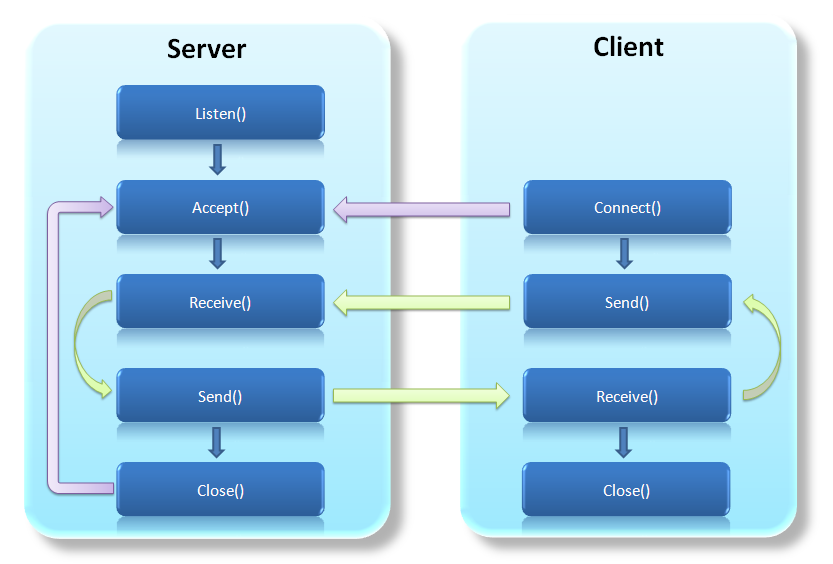
\includegraphics[width=14cm]{images/socket_client_server.png}

\subsection{Các tính năng được xây dựng}
\begin{itemize}
    \item \textbf{Giao diện menu và trò chơi:} Tạo giao diện menu để kết nối socket và khởi động trò chơi. Tạo giao diện trò chơi bao gồm bàn cờ, các ô cờ, con trỏ chuột, kí hiệu đại diện là "X" hoặc "O", hiển thị lượt chơi, tên người chơi và bảng điểm 
    \item \textbf{Kết nối mạng socket:} Mỗi người chơi sẽ chạy một ứng dụng trên máy tính và một máy host sẽ gọi là Server và máy còn lại kết nối với host phải cùng địa chỉ mạng thông qua socket sẽ là Client để gửi và nhận dữ liệu qua lại.
    \item \textbf{Xử lí các nước đi:} Khi người chơi thực hiện một nước đi, Client sẽ gửi thông tin về nước đi đến Server, sau đó Server kiểm tra tính hợp lệ của nước đi và cập nhật trạng thái bàn cờ và điều tương tự được thực hiện khi gửi thông tin về nước đi từ Server đến Client.
    \item \textbf{Kiểm tra chiến thắng:} Mỗi lượt nước đi của người chơi chương trình sẽ kiểm tra xem có tạo thành dãy đủ hàng ngang, hàng dọc hoặc đường chéo để xác định người chiến thắng và tạm dùng cuộc chơi ở cả 2 phía.
    \item \textbf{Xử lí lượt đi lần lượt:} Mỗi lượt nước đi của người chơi sau khi kiểm tra chiến thắng và không đủ điều kiện thắng thì sẽ thay đổi lượt và thông báo cho cả 2 người chơi biết lượt đi tiếp theo là của ai.
    \item \textbf{Gửi thông báo và ghi nhận điểm số:} Khi một người chơi chiến thắng, chương trình sẽ gửi thông báo tới cả hai người chơi để thông báo kết quả và chấm dứt trò chơi. Sau khi bắt đầu lại trò chơi, chương trình sẽ ghi nhận lại điểm số cho người chơi chiến thắng tương ứng.
\end{itemize}
\subsection{Flowchart}
\vspace{-20pt}
\begin{figure}[H]
    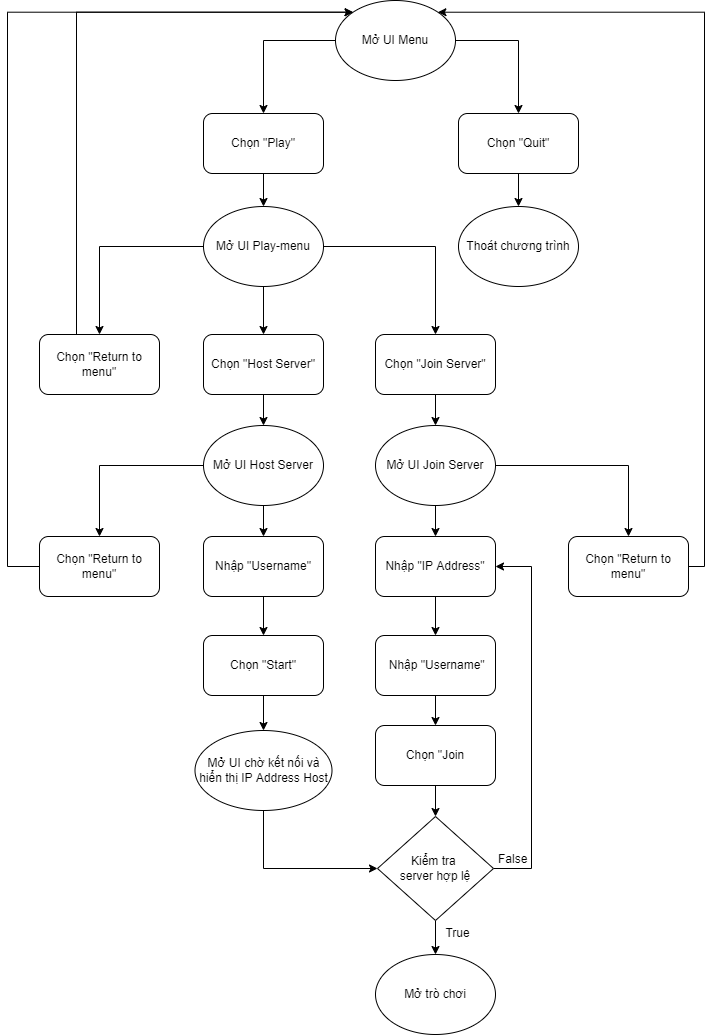
\includegraphics[width=14cm, height=20cm]{images/menu_flowchart.png}
    \caption*{Sơ đồ luồng dữ liệu menu}
\end{figure}

\begin{figure}[H]
    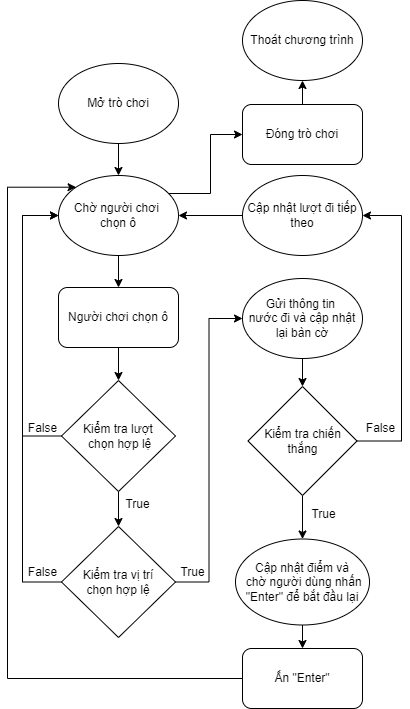
\includegraphics[width=14cm, height=20cm]{images/game_flowchart.png}
    \caption*{Sơ đồ luồng dữ liệu trò chơi}
\end{figure}

\newpage

\section*{PHẦN 3: KẾT QUẢ THỰC HIỆN}
\addcontentsline{toc}{section}{PHẦN 3: KẾT QUẢ THỰC HIỆN}
\setcounter{section}{3}
\setcounter{subsection}{0}
\subsection{Giao diện menu và trò chơi}
\subsubsection{Giao diện menu}
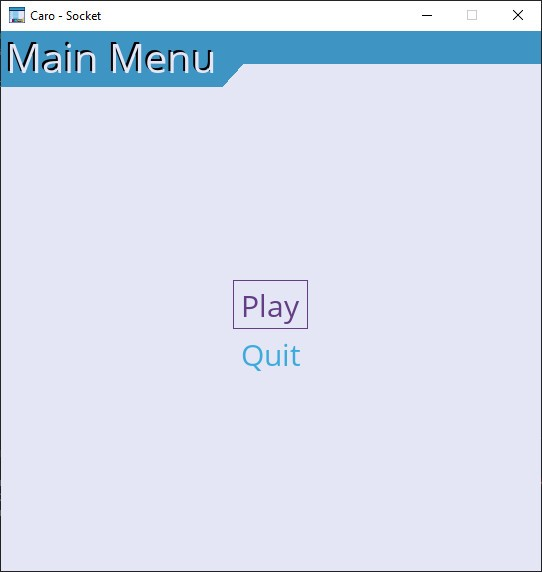
\includegraphics[width=14cm]{images/app/main_menu.png}

\subsubsection{Giao diện trò chơi}
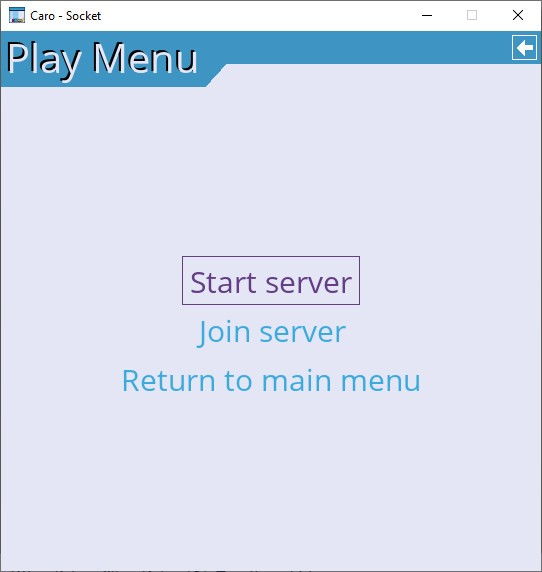
\includegraphics[width=14cm]{images/app/play_menu.png}
\subsection{Kết nối mạng socket}
\subsubsection{Host Server}
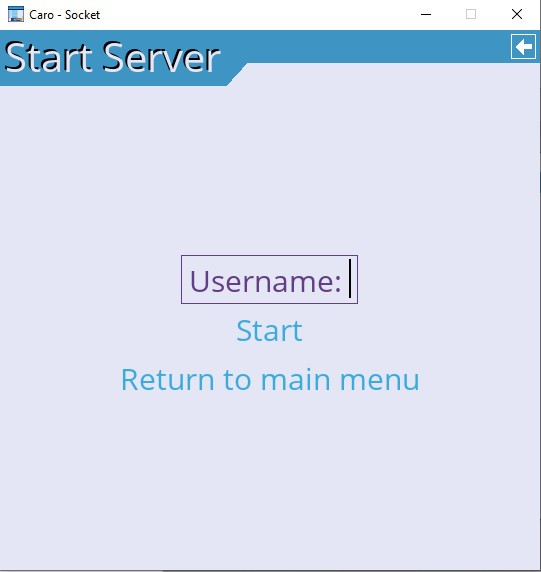
\includegraphics[width=7cm]{images/app/start_server1.png}
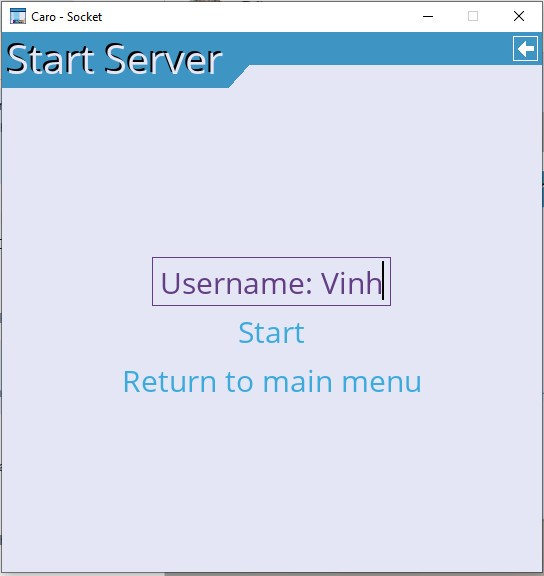
\includegraphics[width=7cm]{images/app/start_server2.png}
\vspace{5pt}

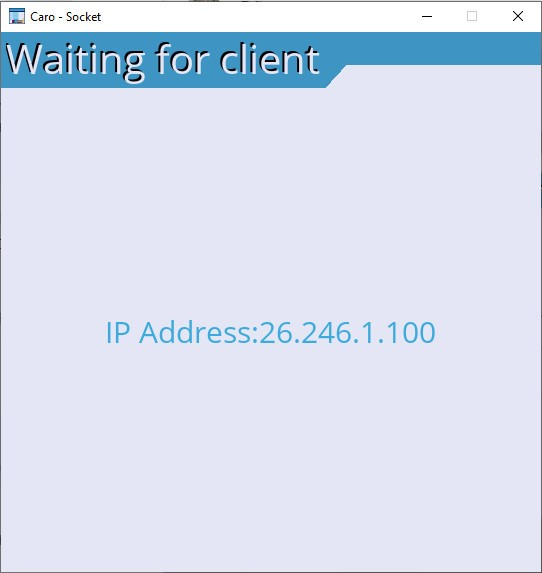
\includegraphics[width=13.5cm, height=10cm]{images/app/waiting_for_client.png}

\subsubsection{Join Server}
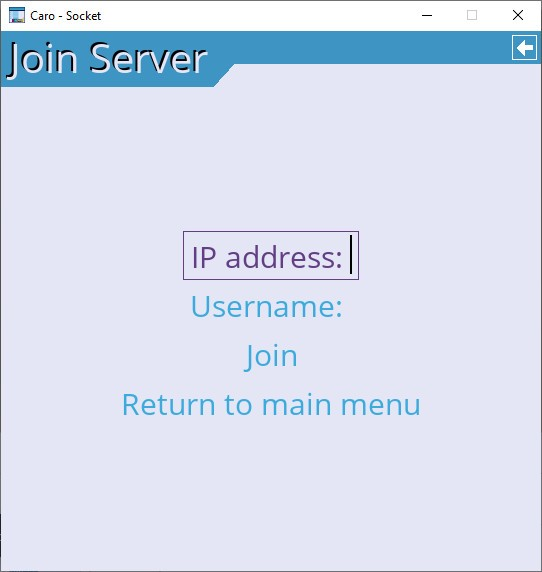
\includegraphics[width=7cm]{images/app/join_server1.png}
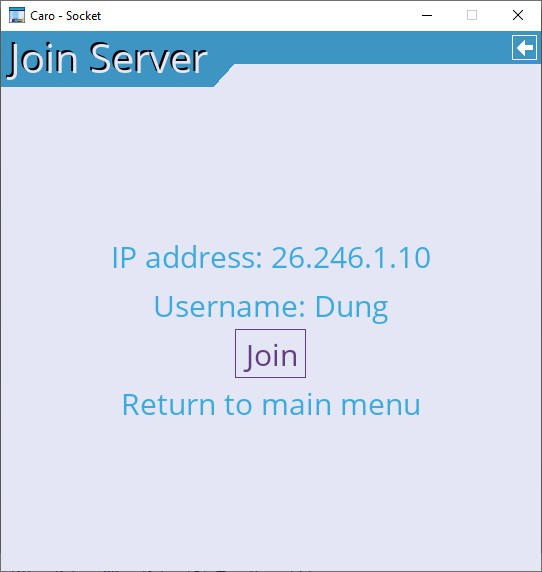
\includegraphics[width=7cm]{images/app/join_server2.png}

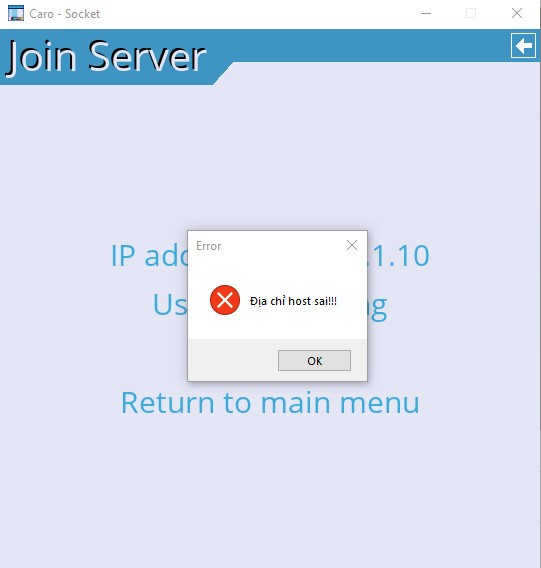
\includegraphics[width=13.5cm, height=10cm]{images/app/join_server3.png}

\subsection{Xử lí các nước đi}
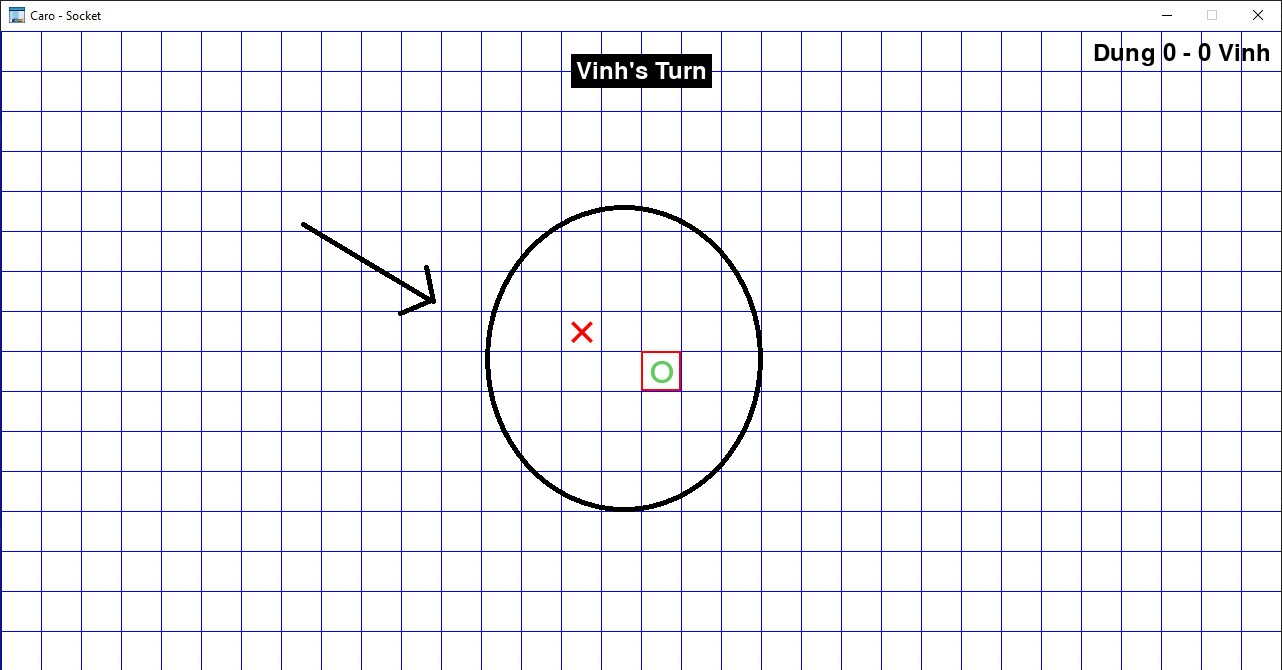
\includegraphics[width=7cm]{images/app/xuly_luotdi1.png}
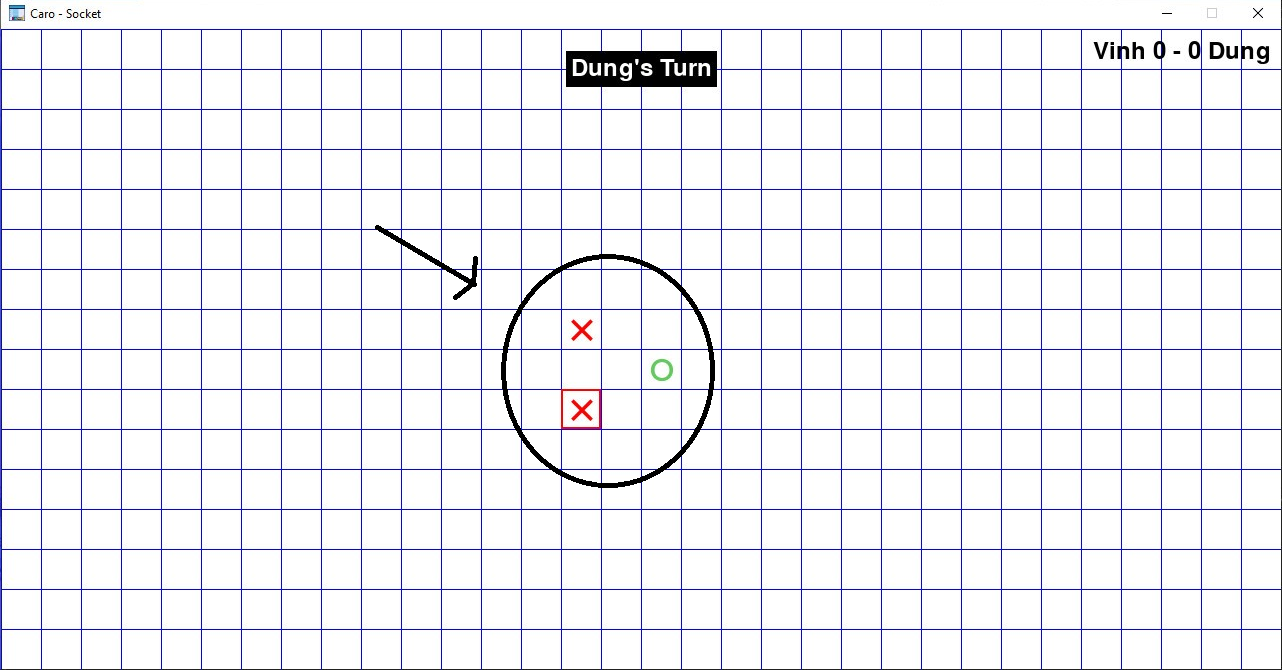
\includegraphics[width=7cm]{images/app/xuly-luotdi2.png}

\subsection{Xử lí lượt đi lần lượt}
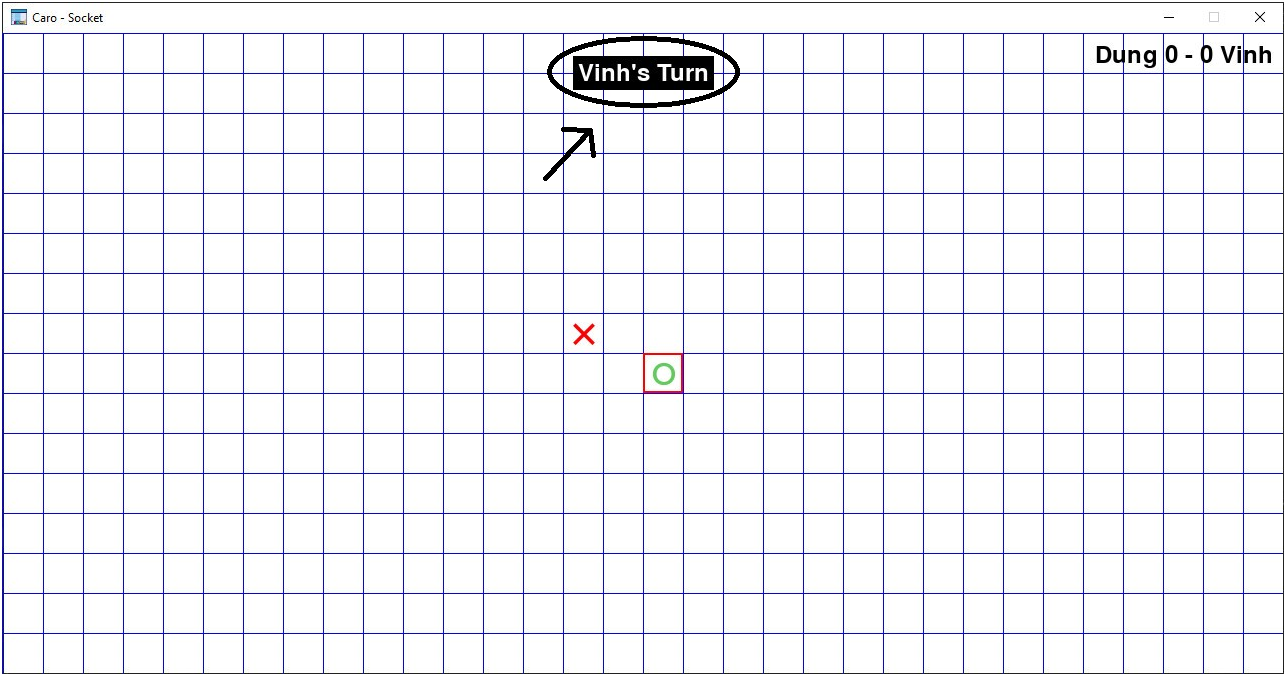
\includegraphics[width=7cm]{images/app/xuly_buocdi1.png}
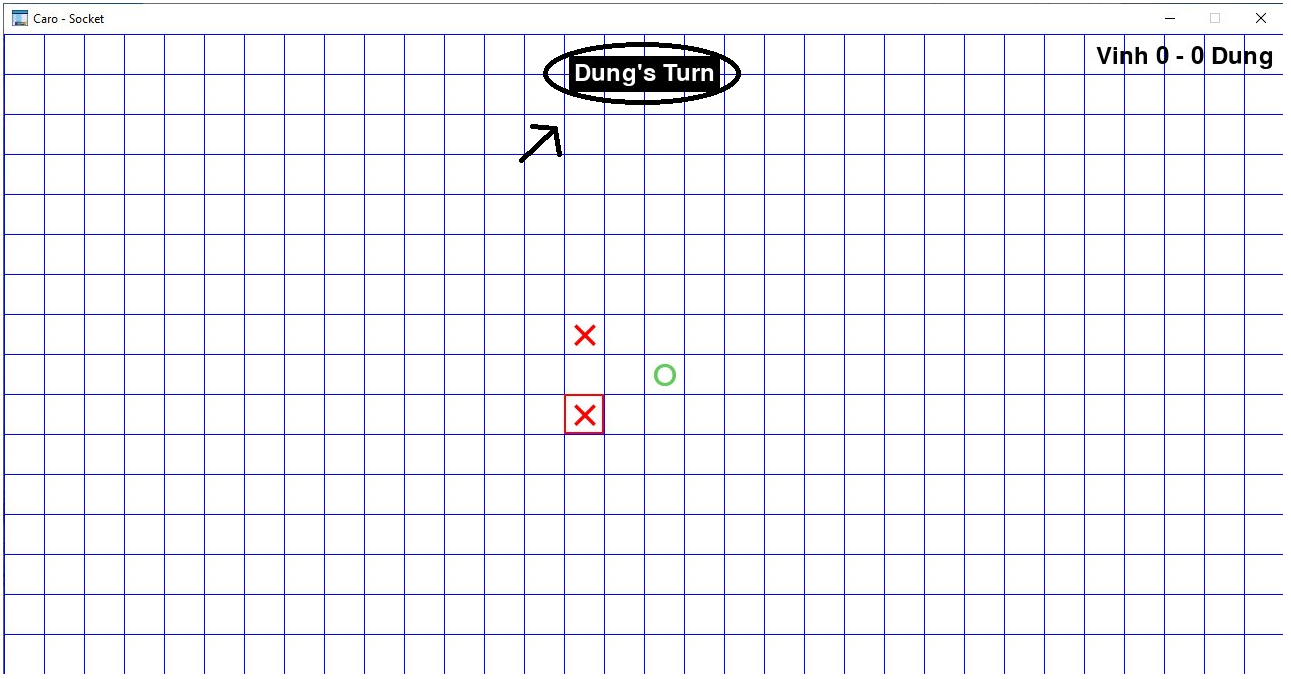
\includegraphics[width=7cm]{images/app/xuly_buocdi2.png}

\subsection{Kiểm tra chiến thắng}

\begin{quotation}
    Check khi đánh thằng bằng hàng dọc
\end{quotation} 
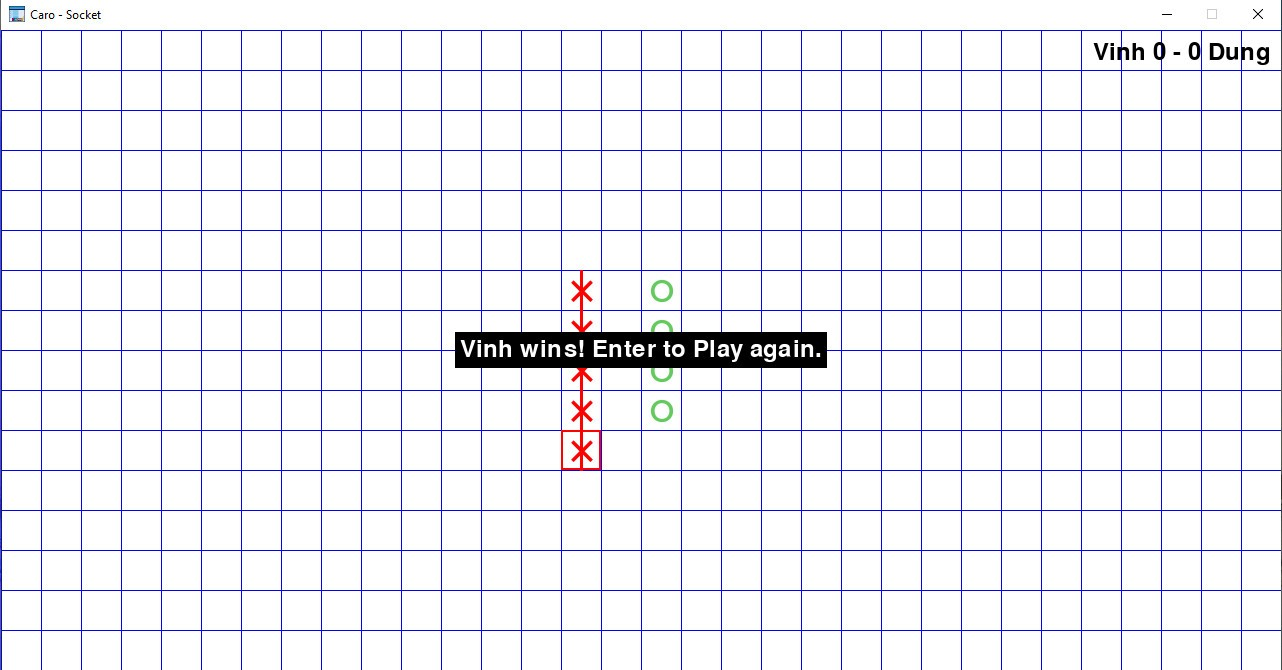
\includegraphics[width=14cm]{images/app/check_vertical.png}
\begin{quotation}
    Check khi đánh thằng bằng hàng ngang
\end{quotation} 
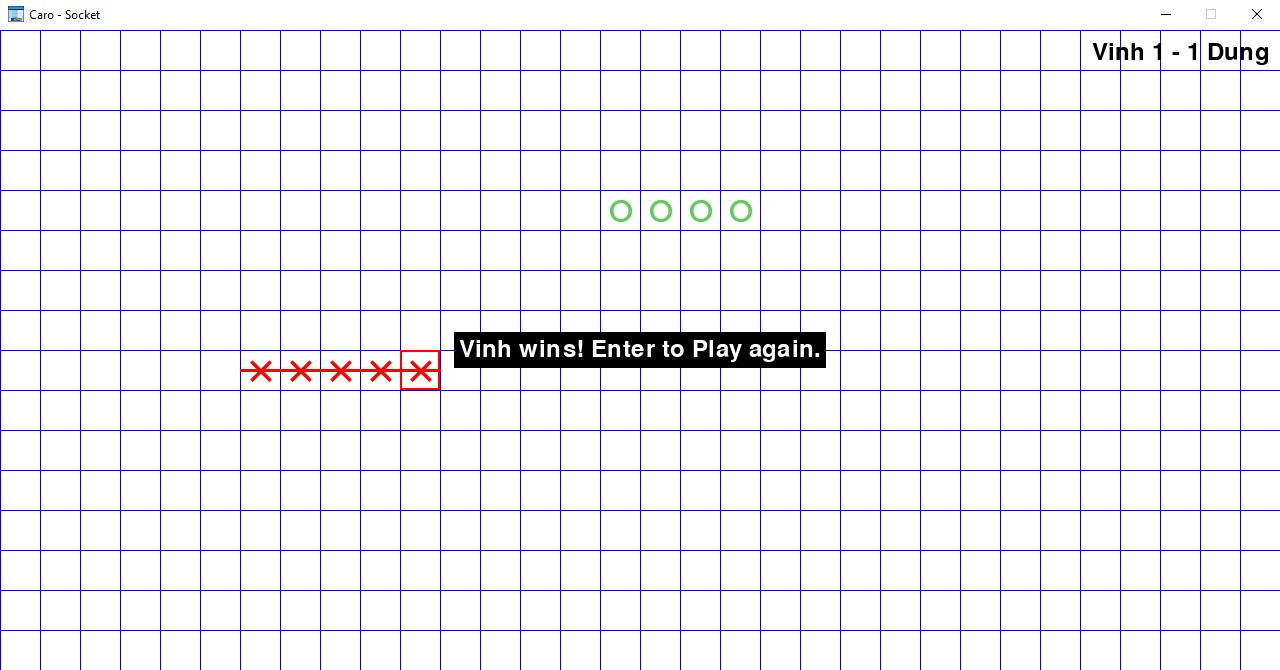
\includegraphics[width=14cm]{images/app/check_horizal.png}
\begin{quotation}
    Check khi đánh thằng bằng hàng chéo
\end{quotation}
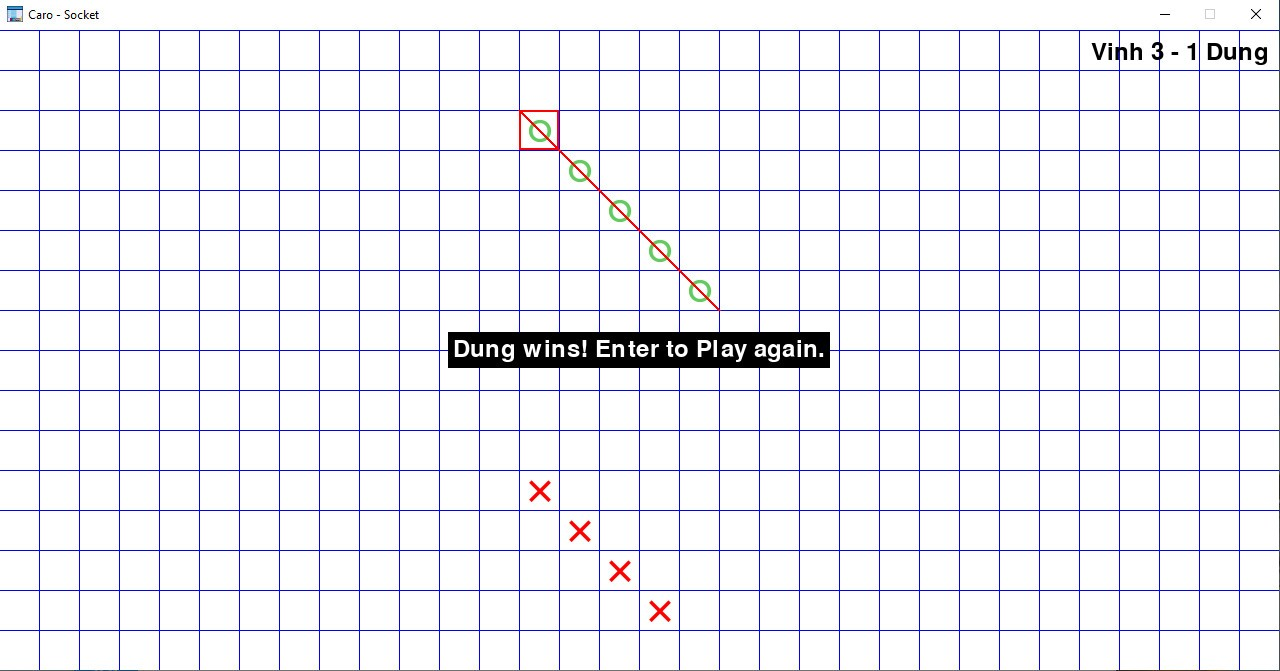
\includegraphics[width=14cm]{images/app/check_cheo.png}


\subsection{Gửi thông báo và ghi nhận điểm số}
\subsubsection{Gửi thông báo}
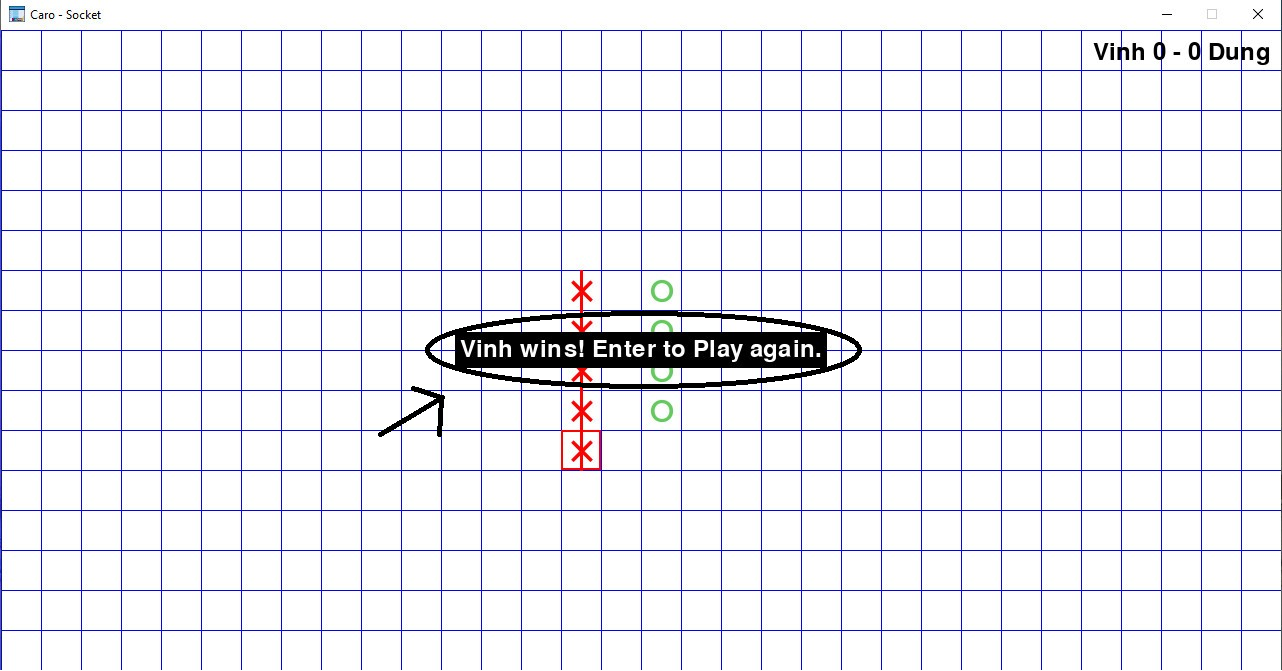
\includegraphics[width=14cm]{images/app/check_win.png}

\subsubsection{Ghi nhận điểm số}
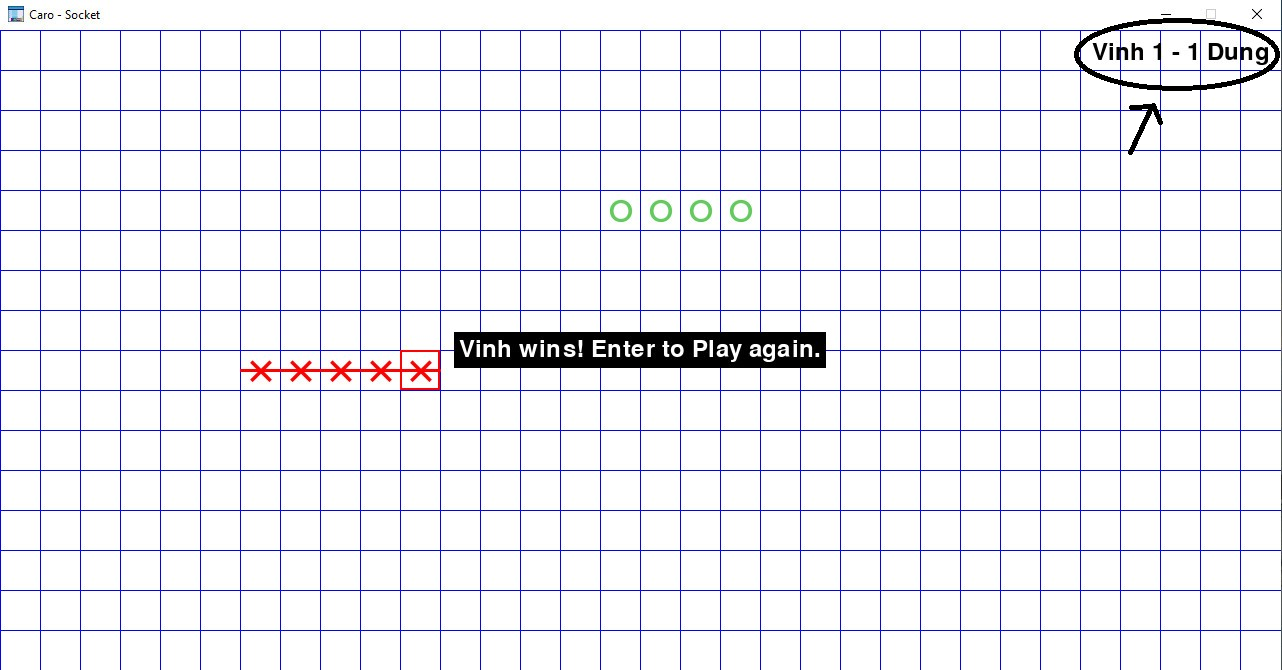
\includegraphics[width=14cm]{images/app/check_score.png}

\newpage
\section*{PHẦN 4: HƯỚNG DẪN CÀI ĐẶT ỨNG DỤNG VÀ MÔI TRƯỜNG}
\addcontentsline{toc}{section}{PHẦN 4: HƯỚNG DẪN CÀI ĐẶT ỨNG DỤNG VÀ MÔI TRƯỜNG}
\setcounter{section}{4}
\setcounter{subsection}{0}

\subsection*{Bước 1: Tải xuống source-code từ GitHub}
\begin{par}
    Tải xuống source-code từ GitHub thông qua đường dẫn sau: \\
    \href{https://github.com/DungIT2k2/Caro-Socket}{https://github.com/DungIT2k2/Caro-Socket} \\
    Giải nén và thu được thư mục game Caro.
\end{par}
\subsection*{Bước 2: Cài đặt python với hệ điều hành tương thích}
\begin{par}
\textbf{Đối với Windows:}  
\begin{itemize}
    \item Truy cập đường dẫn sau: \href{https://www.python.org/downloads/}{https://www.python.org/downloads/}
    \item Tải file .exe và tiến hành cài đặt trên máy tính.
\end{itemize} 
\textbf{Đối với Ubuntu:}
\begin{itemize}
    \item Mở Terminal và nhập lệnh:
    \settowidth{\mylistingwidth}{\ttfamily sudo apt install python3}
    \begin{lstlisting}
sudo apt install python3
    \end{lstlisting}
    
    \item Tiếp theo tiến hành cài đặt pip:
    \settowidth{\mylistingwidth}{\ttfamily sudo apt install -y python3-pip}
    \begin{lstlisting}
sudo apt install -y python3-pip
    \end{lstlisting}
    
    \item Nâng cấp pip mới nhất và cài đặt ifconfig bằng lệnh:
    \settowidth{\mylistingwidth}{\ttfamily pip3 install --upgrade pip }
    \begin{lstlisting}
pip3 install --upgrade pip
    \end{lstlisting}
    
    \settowidth{\mylistingwidth}{\ttfamily sudo apt install net-tools}
    \begin{lstlisting}
sudo apt install net-tools
    \end{lstlisting}
\end{itemize}
\end{par}

\subsection*{Bước 3: Cài đặt các thư viện cần thiết}
\begin{par}
    Mở Terminal trong thư mục Caro, và tiến hành cài đặt thư viện \\
    \textbf{Đối với Windows:}
    \begin{itemize}
        \item Sử dụng lệnh:
        \settowidth{\mylistingwidth}{\ttfamily pip install -r requirements.txt}
    \begin{lstlisting}
pip install -r requirements.txt
    \end{lstlisting}
    \end{itemize}
    \textbf{Đối với Ubuntu:}
    \begin{itemize}
        \item Sử dụng lệnh:
        \settowidth{\mylistingwidth}{\ttfamily pip3 install -r requirements.txt}
    \begin{lstlisting}
pip3 install -r requirements.txt
    \end{lstlisting}
        \item Cài đặt thêm thư viện "tk":
        \settowidth{\mylistingwidth}{\ttfamily sudo apt install python3-tk}
    \begin{lstlisting}
sudo apt install python3-tk
    \end{lstlisting}
    \end{itemize}
\end{par}

\subsection*{Bước 4: Chạy ứng dụng}
\begin{par}
    Tiến hành chạy ứng dụng trên hệ điều hành tương thích. \\
    \textbf{Đối với Windows:}
    \begin{itemize}
        \item Sử dụng lệnh:
        \settowidth{\mylistingwidth}{\ttfamily python run.py}
    \begin{lstlisting}
python run.py
    \end{lstlisting}
    \end{itemize}
    \textbf{Đối với Ubuntu:}
    \begin{itemize}
        \item Sử dụng lệnh:
        \settowidth{\mylistingwidth}{\ttfamily python3 run.py}
    \begin{lstlisting}
python3 run.py
    \end{lstlisting}
    \end{itemize}
\end{par}



\newpage

\section*{NHIỆM VỤ VÀ VAI TRÒ CỦA TỪNG THÀNH VIÊN}
\addcontentsline{toc}{section}{NHIỆM VỤ VÀ VAI TRÒ CỦA TỪNG THÀNH VIÊN}
\subsection*{Thành viên 1: Nguyễn Văn Tiến Dũng - 3120410084}
\begin{itemize}
    \item Thiết kế giao diện trò chơi
    \item Xây dựng socket Client-Server
    \item Xử lí logic nước đi, lượt đi và kết nối đến socket
    \item Viết báo cáo bằng Latex.
\end{itemize}

\subsection*{Thành viên 2: Lai Quang Vinh - 3120410613}
\begin{itemize}
    \item Thiết kế giao diện menu.
    \item Xử lí kiểm tra chiến thắng, ghi điểm và kết nối đến socket
    \item Thiết kế web tĩnh về thông tin chương trình
    \item Viết báo cáo bằng Latex.
\end{itemize}

\newpage
\section*{TÀI LIỆU THAM KHẢO}
\addcontentsline{toc}{section}{TÀI LIỆU THAM KHẢO}
\begin{par}
    \textbf{[1]} Dr. John Hunt.(2019). Advanced Guide to Python 3 Programming, Chapter 12. Nhà xuất bản: Springer \\
    \textbf{[2]} Hướng dẫn xây dựng game Caro cơ bản bằng Python \href{https://www.youtube.com/watch?v=-zZDmxgrhXg}{(Video)} \\
    \textbf{[3]} Tài liệu giới thiệu về pygame-menu \href{https://pygame-menu.readthedocs.io/en/latest/}{(Link)} \\
    \textbf{[4]} (Guide) Socket Programming in Python \href{https://realpython.com/python-sockets/}{(Link)} \\
    \textbf{[5]} Python GUI Programming With Tkinter \href{https://realpython.com/python-gui-tkinter/}{(Link)} \\
    \textbf{[6]} Hướng dẫn kết nối Socket (UDP) cho ứng dụng lần lượt \href{https://www.youtube.com/watch?v=3qlhbez-RPI}{(Video)} 
\end{par}


\end{document}
